\cleardoublepage



\chapter{Réalisation de la solution}

Une fois le problème étudié, et les techniques qui seront utilisées définies, il faut développer la solution pour automatiser le fonctionnement de la machine virtuelle.
\\





%%%%%%%%%%%%%%%%%%%%%%%%%%%%%%%%%%%%%%%%%%%%%%%%%%%%%%%%%%%%%%%%%%%%%%%%%%%%%%%%%%%%%%%%%%%%%%%%%%%%
%%%%%%%%%%%%%%%%%%%%%%%%%%%%%%%%%%%%%%%%%%%%%%%%%%%%%%%%%%%%%%%%%%%%%%%%%%%%%%%%%%%%%%%%%%%%%%%%%%%%
%%%%%%%%%%%%%%%%%%%%%%%%%%%%%%%%%%%%%%%%%%%%%%%%%%%%%%%%%%%%%%%%%%%%%%%%%%%%%%%%%%%%%%%%%%%%%%%%%%%%
%%%%%%%%%%%%%%%%%%%%%%%%%%%%%%%%%%%%%%%%%%%%%%%%%%%%%%%%%%%%%%%%%%%%%%%%%%%%%%%%%%%%%%%%%%%%%%%%%%%%
%%%%%%%%%%%%%%%%%%%%%%%%%%%%%%%%%%%%%%%%%%%%%%%%%%%%%%%%%%%%%%%%%%%%%%%%%%%%%%%%%%%%%%%%%%%%%%%%%%%%

\section{Langage utilisé}

%%%%%%%%%%%%%%%%%%%%%%%%%%%%%%%%%%%%%%%%%%%%%%%%%%%%%%%%%%%%%%%%%%%%%%%%%%%%%%%%%%%%%%%%%%%%%%%%%%%%
%%%%%%%%%%%%%%%%%%%%%%%%%%%%%%%%%%%%%%%%%%%%%%%%%%%%%%%%%%%%%%%%%%%%%%%%%%%%%%%%%%%%%%%%%%%%%%%%%%%%
%%%%%%%%%%%%%%%%%%%%%%%%%%%%%%%%%%%%%%%%%%%%%%%%%%%%%%%%%%%%%%%%%%%%%%%%%%%%%%%%%%%%%%%%%%%%%%%%%%%%

\subsection{Qu'est-ce que Python ?}

\textit{Python}\footnote{Site web : \href{http://www.python.org}{http://www.python.org}} est un langage de programmation récent, créé en 1989 par \href{http://fr.wikipedia.org/wiki/Guido_van_Rossum}{Guido van Rossum}.
Il est codé en Langage C, open-source et gratuit.
De plus, Python est orienté objet, favorisant la programmation impérative structurée, et possède un type dynamique.
Python est \textit{multiplateforme}, c'est à dire qu'il peut être porté aussi bien sur Windows Linux ou Mac OS, mais aussi sur cluster, sans aucune adaptation.
\\


Contrairement aux langages compilés, comme le Langage C ou le C++, Python est un langage \textit{interprété}.
Un programme intermédiaire, appelé \textit{interpréteur}, a pour but d'analyser, de traduire, puis d'exécuter le code source ligne par ligne, qui n'est pas directement exécutable par la machine. 

La machine virtuelle Python permet, comme pour Java ou C\#, de bénéficier du \textit{Ramasse-miettes}, aussi appelé \textit{garbage collector} en anglais, qui permet la gestion de la mémoire.
Lors de l'exécution du programme, celui-ci va allouer de mémoire au fur et à mesure de son exécution.
Lorsque la mémoire allouée n'est plus utilisée, c'est à dire qu'aucun objet n'a de référence sur celle-ci, le garbage collector va libérer la mémoire qui pourra être utilisée par la suite.
\\


C'est un langage de \textit{haut niveau} disposant de nombreux outils, appelés \textit{module}, mis à disposition des programmeurs pour faciliter le développement d'application, dont voici quelques exemples :
\begin{itemize}
	\item[os :] pour l'interaction avec le système d'exploitation ;
	\item[re :] pour l'utilisation des expressions régulières ;
	\item[unittest :] permettant d'effectuer des tests unitaires ;
	\item[threading :] pour l'utilisation de threads.
\end{itemize}
Ils sont comparables aux "packages" du langage Java, ou des "namespace" du C++.

De plus, sa syntaxe est épurée et concise, pour simplifier son utilisation : l'indentation du code source a remplacé les caractères spéciaux, utilisés dans la majorité des langages pour imbriquer les différentes parties du code.
\\




%%%%%%%%%%%%%%%%%%%%%%%%%%%%%%%%%%%%%%%%%%%%%%%%%%%%%%%%%%%%%%%%%%%%%%%%%%%%%%%%%%%%%%%%%%%%%%%%%%%%
%%%%%%%%%%%%%%%%%%%%%%%%%%%%%%%%%%%%%%%%%%%%%%%%%%%%%%%%%%%%%%%%%%%%%%%%%%%%%%%%%%%%%%%%%%%%%%%%%%%%
%%%%%%%%%%%%%%%%%%%%%%%%%%%%%%%%%%%%%%%%%%%%%%%%%%%%%%%%%%%%%%%%%%%%%%%%%%%%%%%%%%%%%%%%%%%%%%%%%%%%

\subsection{Choix de Python}

Python est un langage de plus en plus utilisé dans le monde.
Il dispose de mises-à-jour régulières qui permettent d'améliorer ses performances et sa stabilité, avec l'ajout de fonctionnalités qui le rend très complet.
\\


Ce langage a été choisi par Hutchinson pour le développement de nombreux logiciels car il offre de nombreux modules scientifiques très utilisés dans le centre de recherche, comme par exemple :
\begin{itemize}
	\item NumPy : destiné à la manipulation de matrices et de tableaux multidimensionnels ;
	\item matplotlib : permettant le tracé de graphiques 2D ou 3D.
\end{itemize}
De plus, il permet de s'interfacer avec de nombreux langages de programmation, comme le Fortran ou le C++ très utilisés pour le développements d'applications scientifiques.

De plus, Python est utilisé sur le cluster de calcul de l'entreprise, donc l'intégration de programme Python devient alors très facile.
\\


Le projet sera donc développé dans ce langage, en utilisant les différents modules disponibles et utilisés par Hutchinson.
\\





%%%%%%%%%%%%%%%%%%%%%%%%%%%%%%%%%%%%%%%%%%%%%%%%%%%%%%%%%%%%%%%%%%%%%%%%%%%%%%%%%%%%%%%%%%%%%%%%%%%%
%%%%%%%%%%%%%%%%%%%%%%%%%%%%%%%%%%%%%%%%%%%%%%%%%%%%%%%%%%%%%%%%%%%%%%%%%%%%%%%%%%%%%%%%%%%%%%%%%%%%
%%%%%%%%%%%%%%%%%%%%%%%%%%%%%%%%%%%%%%%%%%%%%%%%%%%%%%%%%%%%%%%%%%%%%%%%%%%%%%%%%%%%%%%%%%%%%%%%%%%%
%%%%%%%%%%%%%%%%%%%%%%%%%%%%%%%%%%%%%%%%%%%%%%%%%%%%%%%%%%%%%%%%%%%%%%%%%%%%%%%%%%%%%%%%%%%%%%%%%%%%
%%%%%%%%%%%%%%%%%%%%%%%%%%%%%%%%%%%%%%%%%%%%%%%%%%%%%%%%%%%%%%%%%%%%%%%%%%%%%%%%%%%%%%%%%%%%%%%%%%%%

\section{Les tests unitaires}

Un des inconvénients du langage interprété est le fait qu'il n'analyse que les lignes de codes au moment de l'exécution.
De plus, le typage dynamique peut lever des erreurs.
De ce fait, il devient difficile de déceler les erreurs situées dans les portions de code peu appelées (notamment la gestion des cas particuliers), comme par exemple un nom de fonction invalide, un argument manquant, ou une variable inexistante.
\\


Les tests unitaires permettent de vérifier le bon fonctionnement d'un programme, ou d'une de ses parties.
Cela consiste à s'assurer que le programme a le comportement attendu, quelque soit la situation dans lequel il se trouve.
Les tests doivent être effectués de manière isolée (ne pas dépendre des autres fonctions non-testées), et automatique.

Par exemple, lors d'une copie de fichier, il faut vérifier que la fonction (ou méthode) appelée lèvera bien une exception lorsque :
\begin{itemize}
	\item le fichier d'entrée est inexistant ;
	\item le répertoire cible est inexistant ;
	\item les droits d'accès sont insuffisants ;
	\item la copie est un échec.
\\
\end{itemize}


Pour minimiser les risques d'erreurs, des tests unitaires ont été développés, permettant de vérifier le bon comportement de l'application dans les différents cas particuliers.
La "bonne pratique" des tests unitaires impose d'utiliser un fichier par classe testée, contenant une classe par méthode, et ayant une méthode par cas particulier.

J'ai utilisé le module \textit{PyUnit}, intégrant de nombreuses classes et méthodes permettant d'effectuer des tests unitaires de manière simple et rapide.
Cela m'a permis de corriger de nombreux bugs, notamment dans l'utilisation des scripts Shell envoyés à la machine virtuelle.
\\





%%%%%%%%%%%%%%%%%%%%%%%%%%%%%%%%%%%%%%%%%%%%%%%%%%%%%%%%%%%%%%%%%%%%%%%%%%%%%%%%%%%%%%%%%%%%%%%%%%%%
%%%%%%%%%%%%%%%%%%%%%%%%%%%%%%%%%%%%%%%%%%%%%%%%%%%%%%%%%%%%%%%%%%%%%%%%%%%%%%%%%%%%%%%%%%%%%%%%%%%%
%%%%%%%%%%%%%%%%%%%%%%%%%%%%%%%%%%%%%%%%%%%%%%%%%%%%%%%%%%%%%%%%%%%%%%%%%%%%%%%%%%%%%%%%%%%%%%%%%%%%
%%%%%%%%%%%%%%%%%%%%%%%%%%%%%%%%%%%%%%%%%%%%%%%%%%%%%%%%%%%%%%%%%%%%%%%%%%%%%%%%%%%%%%%%%%%%%%%%%%%%
%%%%%%%%%%%%%%%%%%%%%%%%%%%%%%%%%%%%%%%%%%%%%%%%%%%%%%%%%%%%%%%%%%%%%%%%%%%%%%%%%%%%%%%%%%%%%%%%%%%%

\section{La documentation}

Documenter le code source est une pratique très importe dans le développement d'une application.
Cela peut s'avérer extrêmement pratique pour la maintenance d'un programme, car le développeur explique son fonctionnement, mais cela devient indispensable pour les utilisateurs qui utiliseront par exemple une bibliothèque existante.
On dit parfois qu'\og un bon code source doit être compréhensible uniquement avec les commentaires \fg.

L'application développée durant le stage pourrait être utilisée ou améliorée à l'avenir.
Il est donc impératif de faciliter sa maintenance, en la documentant correctement.
\\




%%%%%%%%%%%%%%%%%%%%%%%%%%%%%%%%%%%%%%%%%%%%%%%%%%%%%%%%%%%%%%%%%%%%%%%%%%%%%%%%%%%%%%%%%%%%%%%%%%%%
%%%%%%%%%%%%%%%%%%%%%%%%%%%%%%%%%%%%%%%%%%%%%%%%%%%%%%%%%%%%%%%%%%%%%%%%%%%%%%%%%%%%%%%%%%%%%%%%%%%%
%%%%%%%%%%%%%%%%%%%%%%%%%%%%%%%%%%%%%%%%%%%%%%%%%%%%%%%%%%%%%%%%%%%%%%%%%%%%%%%%%%%%%%%%%%%%%%%%%%%%

\subsection{Documentation Python}

Python permet d'intégrer directement la documentation au sein du code source, qui pourra être obtenu dynamiquement lors de l'exécution.
Cela nécessite l'écriture d'une chaine de caractères non référencée au sein de la classe, la méthode ou la fonction.
La documentation pourra ensuite être appelée dynamiquement grâce à l'attribut \lstinline{__doc__}.

Voici un exemple :
\begin{lstlisting}[language=Python]
# Declaration de la fonction avec sa documentation
def maFonction() :
    " Ma documentation "
    pass

# Appel de l'attribut contenant la documentation
if __name__ == '__main__' :
    print maFonction.__doc__
\end{lstlisting}
affichera :
\begin{lstlisting}[language=sh]
Ma documentation
\end{lstlisting}
~~\\


Il existe le module \textit{PyDoc} qui est l'outil de documentation de Python.
Il permet d'afficher la documentation d'un module ou d'une fonction, de manière simple :
\begin{lstlisting}[language=sh]
pydoc <module/>
pydoc <classe>
pydoc <methode/fonction>
\end{lstlisting}
~~\\




%%%%%%%%%%%%%%%%%%%%%%%%%%%%%%%%%%%%%%%%%%%%%%%%%%%%%%%%%%%%%%%%%%%%%%%%%%%%%%%%%%%%%%%%%%%%%%%%%%%%
%%%%%%%%%%%%%%%%%%%%%%%%%%%%%%%%%%%%%%%%%%%%%%%%%%%%%%%%%%%%%%%%%%%%%%%%%%%%%%%%%%%%%%%%%%%%%%%%%%%%
%%%%%%%%%%%%%%%%%%%%%%%%%%%%%%%%%%%%%%%%%%%%%%%%%%%%%%%%%%%%%%%%%%%%%%%%%%%%%%%%%%%%%%%%%%%%%%%%%%%%

\subsection{Doxygen}

\textit{Doxygen}\footnote{Doxygen - Site web : \href{http://www.doxygen.org}{http://www.doxygen.org}} est un programme qui permet de générer une documentation à partir du code source d'une application.
De nombreux langages peuvent être analysés : Langage C, C++, Java, Python, \ldots
La documentation peut être générée dans de nombreux formats : HTML, PDF, LaTeX, \ldots
Doxygen est gratuit et open-source, et est compatible pour les différents systèmes d'exploitation (Windows, Linux, \ldots).
Ce programme est le plus utilisé par les différents développeurs, du fait de ses nombreuses fonctionnalités et sa facilité d'utilisation.
\\


Pour que le programme considère un commentaire comme un "commentaire doxygen", il est nécessaire de respecter certaines règles d'écriture, telles que l'utilisation du symbole "@" ou "$\backslash$" suivi d'un mot clé, ou la délimitation du bloc de commentaire car le double symbole "**" (selon le langage de programmation utilisé).
\\


\begin{lstlisting}[language=C++]
/**
* @details Classe representant une coordonnee dans l'espace.
* @author Julien
*/
class Point {
    /**
    * @brief Constructeur.
    * @param x Abscisse
    * @param y Ordonnee
    */
    Point( int x, int y ) {
        ...
    }
}
\end{lstlisting}
~~\\




%%%%%%%%%%%%%%%%%%%%%%%%%%%%%%%%%%%%%%%%%%%%%%%%%%%%%%%%%%%%%%%%%%%%%%%%%%%%%%%%%%%%%%%%%%%%%%%%%%%%
%%%%%%%%%%%%%%%%%%%%%%%%%%%%%%%%%%%%%%%%%%%%%%%%%%%%%%%%%%%%%%%%%%%%%%%%%%%%%%%%%%%%%%%%%%%%%%%%%%%%
%%%%%%%%%%%%%%%%%%%%%%%%%%%%%%%%%%%%%%%%%%%%%%%%%%%%%%%%%%%%%%%%%%%%%%%%%%%%%%%%%%%%%%%%%%%%%%%%%%%%

\subsection{Filtre d'entrée}

Doxygen nécessite d'utiliser la documentation avant la déclaration de la fonction, alors que Python requiert la documentation à l'intérieur de celle-ci.
Il est donc impossible d'utiliser directement Doxygen pour générer la documentation d'un programme Python.

Il est toutefois possible d'utiliser un \textit{filtre d'entrée} pour le programme Doxygen, qui va formater les commentaires du code source conformément aux règles imposées par Doxygen.
Cela permet donc de générer la documentation de langages de programmation qui possède des règles différentes de celles imposées par Doxygen.

\textit{DoxyPy}\footnote{DoxyPy - Site web et source : \href{http://pypi.python.org/pypi/doxypy/0.3}{http://pypi.python.org/pypi/doxypy/0.3}} est le filtre, gratuit et open-source, programmé en Python, que j'utiliserai pour générer la documentation de mon code avec Doxygen.
\\


De cette façon, la documentation possèdera les avantages des deux méthodes : la documentation peut être utilisable dynamiquement en utilisant l'attribut spécial, en ligne de commande grâce à PyDoc, ou bien être exportable hors du code-source avec Doxygen.
\\





%%%%%%%%%%%%%%%%%%%%%%%%%%%%%%%%%%%%%%%%%%%%%%%%%%%%%%%%%%%%%%%%%%%%%%%%%%%%%%%%%%%%%%%%%%%%%%%%%%%%
%%%%%%%%%%%%%%%%%%%%%%%%%%%%%%%%%%%%%%%%%%%%%%%%%%%%%%%%%%%%%%%%%%%%%%%%%%%%%%%%%%%%%%%%%%%%%%%%%%%%
%%%%%%%%%%%%%%%%%%%%%%%%%%%%%%%%%%%%%%%%%%%%%%%%%%%%%%%%%%%%%%%%%%%%%%%%%%%%%%%%%%%%%%%%%%%%%%%%%%%%
%%%%%%%%%%%%%%%%%%%%%%%%%%%%%%%%%%%%%%%%%%%%%%%%%%%%%%%%%%%%%%%%%%%%%%%%%%%%%%%%%%%%%%%%%%%%%%%%%%%%
%%%%%%%%%%%%%%%%%%%%%%%%%%%%%%%%%%%%%%%%%%%%%%%%%%%%%%%%%%%%%%%%%%%%%%%%%%%%%%%%%%%%%%%%%%%%%%%%%%%%

\section{L'interface graphique}

L'interface graphique est la méthode la plus efficace pour un utilisateur de s'interfacer avec un programme.
Si l'on prend l'exemple de VirtualBox, il est beaucoup plus facile d'utiliser son interface graphique (capture d'écran \ref{Interface graphique de VirtualBox}), que d'utiliser le programme en ligne de commande VBoxManage (partie \ref{VBoxManage}).
\\




%%%%%%%%%%%%%%%%%%%%%%%%%%%%%%%%%%%%%%%%%%%%%%%%%%%%%%%%%%%%%%%%%%%%%%%%%%%%%%%%%%%%%%%%%%%%%%%%%%%%
%%%%%%%%%%%%%%%%%%%%%%%%%%%%%%%%%%%%%%%%%%%%%%%%%%%%%%%%%%%%%%%%%%%%%%%%%%%%%%%%%%%%%%%%%%%%%%%%%%%%
%%%%%%%%%%%%%%%%%%%%%%%%%%%%%%%%%%%%%%%%%%%%%%%%%%%%%%%%%%%%%%%%%%%%%%%%%%%%%%%%%%%%%%%%%%%%%%%%%%%%

\subsection{wxPython}

Comme la solution a été développée dans le langage Python, l'interface graphique sera donc développée dans ce langage, pour faciliter au maximum son intégration.

Il existe différents modules permettant de développer une interface graphique, dont les quatre plus utilisés sont :
\begin{itemize}
	\item \href{http://wiki.python.org/moin/TkInter}{Tkinter} : pour Tk ;
	\item \href{http://www.pygtk.org}{pyGTK} : pour GTK+ ;
	\item \href{http://wiki.python.org/moin/PyQt}{pyQT} : pour Qt ;
	\item \href{http://wxpython.org}{wxPython} : pour wxWidgets.
\end{itemize}

J'utiliserai wxPython, car c'est le module utilisé dans le centre de recherche informatique pour développer les interfaces graphiques en Python.
De plus, il permet d'intégrer d'autres modules de traçage de courbes 2D ou 3D.
\\


Le module \textit{wxPython}\footnote{wxPython - Site web : \href{http://wxpython.org}{http://wxpython.org}} est libre, multiplateforme.
Il implémente \href{http://www.wxwidgets.org/}{wxWidgets} (anciennement wxWindows), qui est aussi une bibliothèque graphique libre, multiplateforme et développée en C++.
Contrairement aux bibliothèques qui restituent la même interface, wxWidgets (et donc wxPython) utilisera l'apparence native de l'environnement sur lequel il est exécuté.

Comme pour Python, wxPython permet une programmation et une gestion des événements simplifiée.
Le développement repose sur l'utilisation de \textit{sizers}, une sorte de tableau permettant le positionnement des objets de manière ordonnée les uns par rapport aux autres dans la fenêtre.
\\




%%%%%%%%%%%%%%%%%%%%%%%%%%%%%%%%%%%%%%%%%%%%%%%%%%%%%%%%%%%%%%%%%%%%%%%%%%%%%%%%%%%%%%%%%%%%%%%%%%%%
%%%%%%%%%%%%%%%%%%%%%%%%%%%%%%%%%%%%%%%%%%%%%%%%%%%%%%%%%%%%%%%%%%%%%%%%%%%%%%%%%%%%%%%%%%%%%%%%%%%%
%%%%%%%%%%%%%%%%%%%%%%%%%%%%%%%%%%%%%%%%%%%%%%%%%%%%%%%%%%%%%%%%%%%%%%%%%%%%%%%%%%%%%%%%%%%%%%%%%%%%

\subsection{wxFormBuilder}

%%%%%%%%%%%%%%%%%%%%%%%%%%%%%%%%%%%%%%%%%%%%%%%%%%%%%%%%%%%%%%%%%%%%%%%%%%%%%%%%%%%%%%%%%%%%%%%%%%%%

\subsubsection{Présentation}

\textit{wxFormBuilder}\footnote{wxFormBuilder - Site web : \href{https://launchpad.net/~wxformbuilder}{https://launchpad.net/$\sim$wxformbuilder}} est un logiciel open-source, permettant de générer facilement et rapidement le code source d'une interface graphique.
Il est possible de générer une interface Python, qui utilisera la bibliothèque wxPython, mais aussi C++ ou XRC qui utiliseront la bibliothèque wxWindows.
\\



%%%%%%%%%%%%%%%%%%%%%%%%%%%%%%%%%%%%%%%%%%%%%%%%%%%%%%%%%%%%%%%%%%%%%%%%%%%%%%%%%%%%%%%%%%%%%%%%%%%%

\subsubsection{Fonctionnement}

\begin{figure}[!h]
	\center
	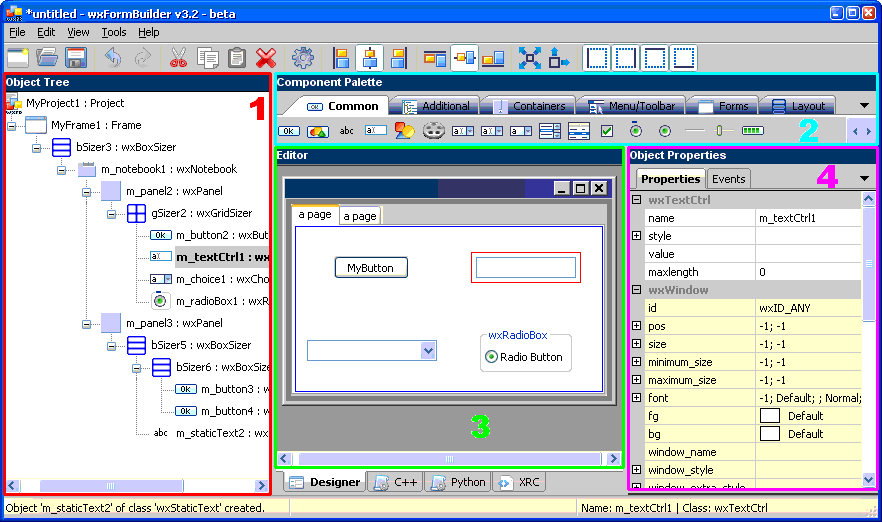
\includegraphics[scale=0.5]{img/wxFormBuilder.png}
	\caption{Interface graphique de wxFormBuilder}
	\label{Interface graphique de wxFormBuilder}
\end{figure}

L'environnement de wxFormBuilder, présenté sur la capture d'écran \ref{Interface graphique de wxFormBuilder}, est composé de 4 grandes parties :
\begin{enumerate}
	\item Object Tree : l'arbre des objets qui présente la disposition des différents éléments les uns dans les autres, notamment avec l'utilisation des Sizers ;
	\item Component Palette : l'ensemble des composants, répertoriés dans leur catégorie. La sélection ;
	\item Editor : l'interface graphique générée, qui permet d'avoir un aperçu de la solution ;
	\item Object Properties : les propriétés de l'objet sélectionné, tels que la taille, la position, son comportement dans le sizer, \ldots
\\
\end{enumerate}


Contrairement à la majorité des éditeurs graphiques, où l'on déplace des composants sur la fenêtre avant de les mettre en forme (taille, position, \ldots), ici la disposition des éléments est définie (uniquement) à l'aide des "layout" qui permettent de structurer la présentation.
\\



%%%%%%%%%%%%%%%%%%%%%%%%%%%%%%%%%%%%%%%%%%%%%%%%%%%%%%%%%%%%%%%%%%%%%%%%%%%%%%%%%%%%%%%%%%%%%%%%%%%%

\subsubsection{Le code généré}

Une des particularités de cet outil, est que le code source généré n'est pas directement exécutable.
Il va générer un fichier (.py, .cpp/.hpp, et/ou .xrc) contenant une (ou plusieurs) classe, qui héritera\footnote{Héritage : principe de la programmation orientée objet, dans lequel les classes "filles" possèderont les mêmes attributs et méthodes que la classe "mère". De plus, elles pourront redéfinir les méthodes héritées, et en définir des nouvelles qui seront spécifiques à sa classe.} d'un objet de base de la bibliothèque.
L'avantage de cette méthode est la possibilité d'utiliser cette classe dans plusieurs projets, sans avoir à dupliquer le code.
\\


wxFormBuilder ne permet que de générer le code source, mais ne permet pas d'y intégrer du code permettant l'initialisation des éléments ou la gestion des événements.
L'interface graphique est alors \textit{statique}, c'est à dire qu'on ne peut pas interagir avec elle : les contrôleurs tels que les "liste-box" ou les "combo-box" seront vides, et ceux du type "bouton" ou "slider" n'auront aucune réaction.

Pour ajouter du dynamisme dans l'application, la technique consiste à créer une nouvelle classe qui héritera de la classe générée par wxFormBuilder.
Ensuite on utilise le polymorphisme d'héritage\footnote{Polymorphisme d'héritage : redéfinition d'une méthode d'une classe héritée pour y ajouter des fonctionnalités ou changer son comportement.} pour y ajouter les différentes initialisations (dans les constructeurs), ainsi que les actions dynamiques (pour les événements).
\\




%%%%%%%%%%%%%%%%%%%%%%%%%%%%%%%%%%%%%%%%%%%%%%%%%%%%%%%%%%%%%%%%%%%%%%%%%%%%%%%%%%%%%%%%%%%%%%%%%%%%
%%%%%%%%%%%%%%%%%%%%%%%%%%%%%%%%%%%%%%%%%%%%%%%%%%%%%%%%%%%%%%%%%%%%%%%%%%%%%%%%%%%%%%%%%%%%%%%%%%%%
%%%%%%%%%%%%%%%%%%%%%%%%%%%%%%%%%%%%%%%%%%%%%%%%%%%%%%%%%%%%%%%%%%%%%%%%%%%%%%%%%%%%%%%%%%%%%%%%%%%%

\subsection{Scinder l'interface}
\label{Scinder l'interface}

%%%%%%%%%%%%%%%%%%%%%%%%%%%%%%%%%%%%%%%%%%%%%%%%%%%%%%%%%%%%%%%%%%%%%%%%%%%%%%%%%%%%%%%%%%%%%%%%%%%%

\subsubsection{Pourquoi ?}

Pour permettre une meilleure maintenance des outils scientifiques, la solution envisagée consistait à utiliser un disque virtuel par outil.

En se basant sur le même principe, j'ai décidé de programmer chaque interface relative à un outil dans des fichiers différents, et l'interface principale afficherait l'outil sélectionné par l'utilisateur de manière dynamique.
\\


Ce choix permettra de ne pas avoir à modifier le code source de l'interface graphique de base lors de la modification d'outils.
Par exemple, pour ajouter un nouvel outil dans la solution, en plus d'ajouter le disque virtuel dans lequel l'outil est installé, il faudra programmer un morceau d'interface graphique (avec les objets et la gestion des événements) dans un fichier que l'on ajoutera aux autres fichiers de la solution.
\\



%%%%%%%%%%%%%%%%%%%%%%%%%%%%%%%%%%%%%%%%%%%%%%%%%%%%%%%%%%%%%%%%%%%%%%%%%%%%%%%%%%%%%%%%%%%%%%%%%%%%

\subsubsection{Règles imposées}

Cette technique impose toutefois certaines règles à respecter aux interfaces de outils pour pouvoir être intégrées à l'interface de base.
Si elles ne sont pas respectées, l'application ne fonctionnera pas.
\\


Dans l'interface de base, l'objet \textit{wxChoicebook} fonctionne de manière similaire aux onglets (objet \textit{wxNotebook}), mais les différents éléments sont proposés sous forme de liste plutôt que sous forme d'onglet.
Il contient un ensemble de panels\footnote{Panel : objet graphique contenant des composants.} (objet \textit{wxPanel}), et le choix dans la liste permet d'afficher le panel correspondant.

L'interface de l'outil doit donc être un objet héritant de la classe \textit{wxPanel} pour pouvoir être intégré à l'interface de base.
\\


Il est possible de changer dynamiquement des modules et des classe en Python.
Le chargement d'un module s'effectue grâce à la fonction spéciale \lstinline{__import__}, qui prend comme argument le nom du module, c'est à dire le nom du fichier sans son extension, et retourne la variable qui représente le module.
Le module doit se trouver dans le \textit{path}\footnote{Path : variable d'environnement permettant d'enregistrer l'emplacement des différents exécutables.} pour être trouvé, on ajoutera donc le répertoire contenant l'ensemble des interfaces des outils dans le path.
On peut ensuite appeler directement le contenu du module à partir de sa variable, à condition que la classe, la fonction ou la variable globale existe.
\begin{lstlisting}[language = sh]
sys.path.append( "chemin du repertoire" )
monModule = __import__( "nom du module" )
monPanel = monModule.MaClasse( arguments )
\end{lstlisting}

L'ensemble les fichiers comportera donc une classe ayant le même nom ("MyPanel" dans mon cas), ainsi que les mêmes arguments, pour pouvoir être appelé dynamiquement.
\\





%%%%%%%%%%%%%%%%%%%%%%%%%%%%%%%%%%%%%%%%%%%%%%%%%%%%%%%%%%%%%%%%%%%%%%%%%%%%%%%%%%%%%%%%%%%%%%%%%%%%
%%%%%%%%%%%%%%%%%%%%%%%%%%%%%%%%%%%%%%%%%%%%%%%%%%%%%%%%%%%%%%%%%%%%%%%%%%%%%%%%%%%%%%%%%%%%%%%%%%%%
%%%%%%%%%%%%%%%%%%%%%%%%%%%%%%%%%%%%%%%%%%%%%%%%%%%%%%%%%%%%%%%%%%%%%%%%%%%%%%%%%%%%%%%%%%%%%%%%%%%%
%%%%%%%%%%%%%%%%%%%%%%%%%%%%%%%%%%%%%%%%%%%%%%%%%%%%%%%%%%%%%%%%%%%%%%%%%%%%%%%%%%%%%%%%%%%%%%%%%%%%
%%%%%%%%%%%%%%%%%%%%%%%%%%%%%%%%%%%%%%%%%%%%%%%%%%%%%%%%%%%%%%%%%%%%%%%%%%%%%%%%%%%%%%%%%%%%%%%%%%%%

\section{Construction des outils}

Comme expliqué plus tôt dans la partie \ref{Solution envisagée}, chaque outil sera installé sur un disque virtuel distinct.
Outre l'avantage du (re)déploiement des outils, cette solution offre certains avantages mais soulève aussi des inconvénients.
De plus leur installation requiert des manipulations supplémentaires.
\\




%%%%%%%%%%%%%%%%%%%%%%%%%%%%%%%%%%%%%%%%%%%%%%%%%%%%%%%%%%%%%%%%%%%%%%%%%%%%%%%%%%%%%%%%%%%%%%%%%%%%
%%%%%%%%%%%%%%%%%%%%%%%%%%%%%%%%%%%%%%%%%%%%%%%%%%%%%%%%%%%%%%%%%%%%%%%%%%%%%%%%%%%%%%%%%%%%%%%%%%%%
%%%%%%%%%%%%%%%%%%%%%%%%%%%%%%%%%%%%%%%%%%%%%%%%%%%%%%%%%%%%%%%%%%%%%%%%%%%%%%%%%%%%%%%%%%%%%%%%%%%%

\subsection{Bibliothèques, paquets et installation}
\label{Bibliothèques, paquets et installation}

Une présentation du mode de fonctionnement des programmes sous Linux permettra de mieux comprendre la méthode d'installation des outils, ainsi que des problèmes rencontrés.
\\



%%%%%%%%%%%%%%%%%%%%%%%%%%%%%%%%%%%%%%%%%%%%%%%%%%%%%%%%%%%%%%%%%%%%%%%%%%%%%%%%%%%%%%%%%%%%%%%%%%%%

\subsubsection{Les bibliothèques}

Aussi appelées \textit{libraries} en anglais, les \textit{bibliothèques} sont des ensembles de fonctions mis à disposition des développeurs, afin de ne pas avoir à les réécrire.
La quasi-totalité des programmes les utilisent et dépendent d'elles pour fonctionner.
\\


Il existe deux types de bibliothèques :

\paragraph{Les bibliothèques dynamiques}
(aussi appelées \textit{partagées}) sont installées sur le système d'exploitation.
Lors de l'exécution d'un programme qui utilise ce type de bibliothèques, elles seront chargées en mémoire avant leur utilisation (voir schéma \ref{Schéma Bibliothèque dynamique}).
Ce programme est alors appelé \textit{programme dynamique}.
L'inconvénient est qu'il est nécessaire que le système possède ces bibliothèques pour pouvoir l'exécuter.

\begin{figure}[!h]
	\center
	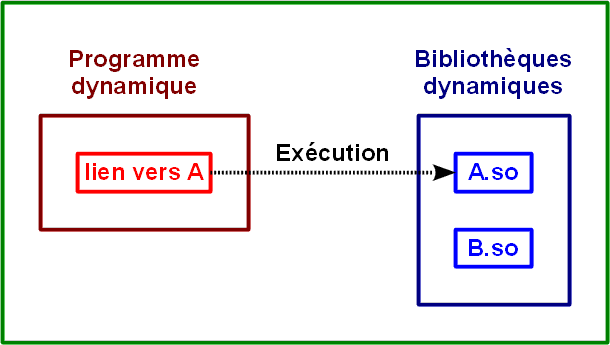
\includegraphics[scale=0.5]{img/Bibliotheque_dynamique.png}
	\caption{Schéma d'un programme dynamique}
	\label{Schéma Bibliothèque dynamique}
\end{figure}


\paragraph{Les bibliothèques statiques}
sont intégrées (par copie) au programme lors de sa compilation (voir schéma \ref{Schéma Bibliothèque statique}).
Le volume de ce programme sera donc plus élevé, car la bibliothèque est copiée à l'intérieur de celui-ci.
L'avantage de cette solution est que le programme sera exécutable sur les différents systèmes, même si la bibliothèque n'y est pas installée.
Ce programme est alors appelé \textit{programme statique}.

\begin{figure}[!h]
	\center
	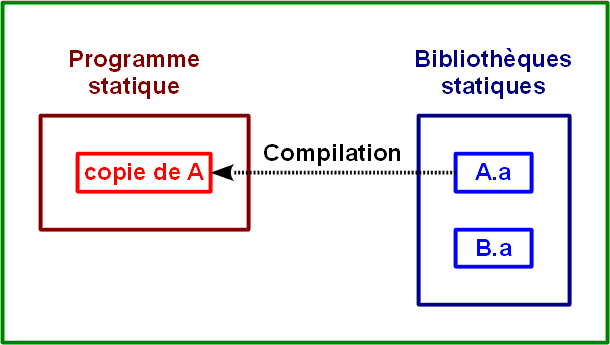
\includegraphics[scale=0.5]{img/Bibliotheque_statique.png}
	\caption{Schéma d'un programme statique}
	\label{Schéma Bibliothèque statique}
\end{figure}

Notons qu'un programme peut utiliser les deux types de bibliothèques.
Il sera alors dynamique, car il dépend de bibliothèques dynamiques, mais possèdera moins de dépendances.
\\


Une bibliothèque se compose de trois parties :
\begin{enumerate}
	\item La partie dynamique (fichiers \textit{.dll} sous Windows et \textit{.so} sous Unix) permet aux programmes (dynamiques) de fonctionner sur le système.
	\item La partie statique (fichiers \textit{.lib} sous Windows et \textit{.a} sous Unix) qui est nécessaire à la compilation de programmes "statique".
Il s'agit des fichiers qui seront intégrés à l'exécutable du programme pour fonctionner de manière autonome.
	\item Les fichiers d'en-tête (fichiers \textit{.h}, appelés \textit{headers} en anglais) nécessaires à la compilation, qui contiennent les prototypes\footnote{Prototype : syntaxe d'une fonction décrivant les paramètres d'entrée ainsi que le retour.} des différentes fonctions de la bibliothèque.
\end{enumerate}
~~\\



%%%%%%%%%%%%%%%%%%%%%%%%%%%%%%%%%%%%%%%%%%%%%%%%%%%%%%%%%%%%%%%%%%%%%%%%%%%%%%%%%%%%%%%%%%%%%%%%%%%%

\subsubsection{Les paquets}

Les paquets (\textit{packages} en anglais) sont l'équivalent des exécutables de Windows (\textit{.exe}).
Il s'agit d'un type d'archives contenant les fichiers et procédures nécessaires à l'installation de programmes ou de bibliothèques.

Dans le cas d'une bibliothèque, le paquet portera le nom de la bibliothèque, précédé par \textit{lib} (par exemple "libtool" pour la bibliothèque "tool").
Dans cette partie \ref{Bibliothèques, paquets et installation}, on confondra programme et bibliothèque.
\\


Selon la distribution utilisée, ils peuvent avoir un format différent :
\begin{itemize}
	\item Les RPM (RedHat Package Manager), d'extension \textit{.rpm}, sont utilisés par les distributions basées sur RedHat dont Fedora ;
C'est le format standard de Linux.
	\item Les DEB, d'extension \textit{.deb}, sont utilisés par les systèmes basés sur la distribution Debian ;
	\item Les archives, d'extension \textit{.tar.gz} ou \textit{.gz} compressés ou non, peuvent contenir les sources de l'application ou les fichiers binaires déjà compilés.
Ils sont généralement compatibles avec les différentes distributions.
\\
\end{itemize}


Outre les différentes versions, les paquets peuvent se présenter sous diverses formes, en fonction de leur contenu :
\begin{itemize}
	\item Les paquets dits "normaux" ne contiennent que la partie dynamique du programme nécessaire à son fonctionnement et ses dépendances.
C'est la forme par défaut.;
	\item Les paquets statiques (\textit{nompaquet-static}) contiennent soit la forme autonome d'un programme, soit la partie statique d'une bibliothèque. ;
	\item Les paquets de développement (\textit{nompaquet-devel}) contiennent l'ensemble des fichiers d'en-tête, permettant la compilation et la réutilisation du paquet ;
	\item D'autres types, plus rares comme par exemple \textit{client} (\textit{nompaquet-client}) et \textit{serveur} (\textit{nompaquet-serveur}) pour le paquet \textit{OpenSSH} qui ne contiennent qu'une partie du programme.
\\
\end{itemize}



%%%%%%%%%%%%%%%%%%%%%%%%%%%%%%%%%%%%%%%%%%%%%%%%%%%%%%%%%%%%%%%%%%%%%%%%%%%%%%%%%%%%%%%%%%%%%%%%%%%%

\subsubsection{L'installation}
\label{L'installation}

Il existe trois méthodes permettant d'installer un programme dans Linux.

\paragraph{Le gestionnaire de paquets}
est un programme permettant le téléchargement (à partir d'un dépôts\footnote{Dépôt : serveur internet sur lequel sont répertoriés les paquets officiels ou non.}) et l'installation de paquets, de manière automatique et transparente.
Les dépendances sont gérées automatiquement : le paquet sera installé avec les différents paquets dont il dépend, si ceux-ci ne sont pas déjà installés sur le système.

Il est utilisé en ligne de commande, mais il existe des programmes utilisant une interface graphique pour faciliter son utilisation.
Sous les systèmes RedHat, sur lequel se base Fedora, le gestionnaire de paquet est \lstinline{yum}, alors que sous les systèmes Debian il s'agit de \lstinline{apt}.
\\


\paragraph{Les paquets}
peuvent être manipulés "à bas niveau", c'est à dire dans l'arborescence de Linux.
Les commandes \lstinline{rpm} sous RedHat ou \lstinline{dpkg} sous Debian, permettent l'installation, l'affichage du contenu ou des informations, \ldots sur un paquet.
Elles permettent aussi de connaitre l'ensemble des paquets installés ou de désinstaller un paquet.
\\


\paragraph{Les archives}
qui ne respectent pas le standard RPM ou DEB doivent être installées manuellement, en suivant le processus détaillé dans le fichier \textit{README} ou \textit{INSTALL}.
Généralement, cela s'effectue en trois étapes :
\begin{enumerate}
	\item Configuration des fichiers qui permettront la compilation, appelés \textit{Makefile}, et vérification de l'état du système (bibliothèques requises installées).
Cela s'effectue à l'aide du script exécutable \textit{configure} situé à la base de l'archive.
	\item Compilation des sources, transformant le code source compréhensible par l'humain exécutable par la machine.
	\item Installation du programme, qui va copier les fichiers binaires dans l'arborescence de Linux.
\end{enumerate}
Les commandes à exécuter sont :
\begin{lstlisting}
$ ./configure
$ make
# make install
\end{lstlisting}
C'est cette méthode qui sera utilisé pour installer les différents outils, car ceux-ci ne sont pas disponibles au format RPM.
\\




%%%%%%%%%%%%%%%%%%%%%%%%%%%%%%%%%%%%%%%%%%%%%%%%%%%%%%%%%%%%%%%%%%%%%%%%%%%%%%%%%%%%%%%%%%%%%%%%%%%%
%%%%%%%%%%%%%%%%%%%%%%%%%%%%%%%%%%%%%%%%%%%%%%%%%%%%%%%%%%%%%%%%%%%%%%%%%%%%%%%%%%%%%%%%%%%%%%%%%%%%
%%%%%%%%%%%%%%%%%%%%%%%%%%%%%%%%%%%%%%%%%%%%%%%%%%%%%%%%%%%%%%%%%%%%%%%%%%%%%%%%%%%%%%%%%%%%%%%%%%%%

\subsection{Disque virtuel individuel}

Le choix d'utiliser un disque virtuel par outil, expliqué dans la partie \ref{Solution envisagée}, impose d'installer l'outil dans le disque virtuel.
\\



%%%%%%%%%%%%%%%%%%%%%%%%%%%%%%%%%%%%%%%%%%%%%%%%%%%%%%%%%%%%%%%%%%%%%%%%%%%%%%%%%%%%%%%%%%%%%%%%%%%%

\subsubsection{Choix du répertoire d'installation}

Il est possible d'installer un programme dans un répertoire spécifique plutôt que de laisser les fichiers s'installer dans les répertoires du système (\textit{/bin}, \textit{/lib}, \ldots).
Pour cela il existe l'option \lstinline{--prefix} au script de configuration (voir partie \ref{L'installation}), en précisant le chemin du répertoire :
\begin{lstlisting}[language = sh]
$ ./configure --prefix=<repertoire>
\end{lstlisting}
Ainsi les différents fichiers et exécutables du programme seront placés dans le répertoire cible : \lstinline{<repertoire>/bin}, \lstinline{<repertoire>/usr}, \lstinline{<repertoire>/lib}, \ldots
\\


Pour installer un outil sur un disque virtuel, il suffit donc de choisir comme répertoire d'installation le répertoire dans lequel est monté le disque virtuel.
\\



%%%%%%%%%%%%%%%%%%%%%%%%%%%%%%%%%%%%%%%%%%%%%%%%%%%%%%%%%%%%%%%%%%%%%%%%%%%%%%%%%%%%%%%%%%%%%%%%%%%%

\subsubsection{Taille minimale}

Une fois installés, les outils ne vont plus générer de fichier dans le répertoire d'installation, hormis les fichiers de sorties qui se trouveront dans un répertoire cible spécifié lors de l'exécution.
Pour minimiser l'espace disque occupé par les différents outils sur le disque dur de la machine hôte, les disques virtuels auront une taille minimale.

Pour connaitre la taille d'une application, il faut effectuer une première installation dans un répertoire ou sur un disque virtuel temporaire.
Une fois installé, la taille totale de l'outil est égale à la taille totale du répertoire d'installation.
\\


Le disque virtuel possède un en-tête et le système des fichiers (voir partie \ref{Les disques virtuels}), qui représentent une certaine taille du disque virtuel.
On laissera alors une marge de quelques MégaOctets sur la taille totale pour éviter tout problème lors de l'installation.
\\




%%%%%%%%%%%%%%%%%%%%%%%%%%%%%%%%%%%%%%%%%%%%%%%%%%%%%%%%%%%%%%%%%%%%%%%%%%%%%%%%%%%%%%%%%%%%%%%%%%%%
%%%%%%%%%%%%%%%%%%%%%%%%%%%%%%%%%%%%%%%%%%%%%%%%%%%%%%%%%%%%%%%%%%%%%%%%%%%%%%%%%%%%%%%%%%%%%%%%%%%%
%%%%%%%%%%%%%%%%%%%%%%%%%%%%%%%%%%%%%%%%%%%%%%%%%%%%%%%%%%%%%%%%%%%%%%%%%%%%%%%%%%%%%%%%%%%%%%%%%%%%

\subsection{Compilation statique}
\label{Compilation statique}

%%%%%%%%%%%%%%%%%%%%%%%%%%%%%%%%%%%%%%%%%%%%%%%%%%%%%%%%%%%%%%%%%%%%%%%%%%%%%%%%%%%%%%%%%%%%%%%%%%%%

\subsubsection{Comparaison statique et dynamique}

Avantages de la compilation dynamique :
\begin{itemize}
	\item Les différentes bibliothèques ne sont pas dupliquées dans les différents outils, mais présentes uniquement dans la machine virtuelle ;
Cela implique que la solution totale sera de taille minimale.
	\item Les disques virtuels seront de petite taille, mais la machine virtuelle de taille plus importante.
Comme on ne déploie qu'une seule fois la machine virtuelle, et qu'il est possible de déployer plusieurs fois le même outil (mise à jour, corrections de bugs, \ldots), alors le déploiement sera plus rapide.
\\
\end{itemize}


Avantages de la compilation statique :
\begin{itemize}
	\item Il est impossible de connaitre à l'avance quelles seront les bibliothèques dont dépendront l'ensemble des outils.
En effet, si un nouvel outil est ajouté à la solution, utilisant une bibliothèque non-installée, alors il sera impossible de l'exécuter ;
	\item L'installation des nombreuses bibliothèques dynamiques sur la machine virtuelle pose plusieurs inconvénients :
		\begin{itemize}
			\item Bien que les paquets sont assez légers (quelques MégaOctets), la machine virtuelle possède une taille limite.
Et il est impossible de modifier sa taille, sauf en cas de maintenance qui nécessiterait de redéployer la solution ;
			\item Les performances du système peu décroitre avec la présence des nombreux paquets.
		\end{itemize}
	\item Il n'est pas nécessaire de posséder une connexion internet pour télécharger les paquets.
\\
\end{itemize}


J'ai décidé de choisir la compilation statique des outils, ce qui permet de simplifier les recherches de dépendances, malgré les disques virtuels de taille plus importante.
\\



%%%%%%%%%%%%%%%%%%%%%%%%%%%%%%%%%%%%%%%%%%%%%%%%%%%%%%%%%%%%%%%%%%%%%%%%%%%%%%%%%%%%%%%%%%%%%%%%%%%%

\subsubsection{La compilation}

Par défaut la compilation d'un programme crée un exécutable dynamique.
Mais il est possible de compiler un programme de façon statique, en utilisant l'option \lstinline{-static} lors de la compilation.

Comme la compilation des outils s'effectue à l'aide des Makefile, générés automatiquement, il faut que cette option soit activée dans celui-ci, et pour toutes les compilations faites.
Pour cela, il existe parfois une option dans le script de configuration (confère partie \ref{L'installation}) permettant d'activer la compilation statique :
\begin{lstlisting}[language = sh]
$ ./configure --disable-shared --enable-static
\end{lstlisting}
Les deux options sont complémentaires : on ne peut activer les deux en même temps.
Lorsqu'une est activée (enable), l'autre est désactivée (disable).
\\


La compilation des outils s'effectue sur la machine virtuelle complète, qui dispose de toutes les bibliothèques statiques nécessaires.
En effectuant la compilation des différents outils, ceux-ci ne sont pas compilés en "statique".
J'ignore l'origine du problème, car les options sont correctes et aucune erreur n'est survenue lors de l'installation.
\\



%%%%%%%%%%%%%%%%%%%%%%%%%%%%%%%%%%%%%%%%%%%%%%%%%%%%%%%%%%%%%%%%%%%%%%%%%%%%%%%%%%%%%%%%%%%%%%%%%%%%

\subsubsection{Solution au problème}
\label{Solution au problème}

Pour connaitre l'ensemble des bibliothèques dynamiques dont dépend un exécutable, il existe la commande \lstinline{ldd}.
A chaque bibliothèque est associé le chemin d'installation, ou "not found" si celle-ci n'est pas installée.
\begin{lstlisting}[language = sh]
$ ldd ./mbdyn

linux-vdso.so.1 =>  (0x00007fff20792000)
liblapack.so.3 => /usr/lib64/atlas/liblapack.so.3 (0x00007fbaaae58000)
libblas.so.3 => /usr/lib64/libblas.so.3 (0x00007fbaaac02000)
libpthread.so.0 => /lib64/libpthread.so.0 (0x0000003217800000)
librt.so.1 => /lib64/librt.so.1 (0x00000037ef600000)
libgfortran.so.3 => /usr/lib64/libgfortran.so.3 (0x00007fbaaa8eb000)
libquadmath.so.0 => /usr/lib64/libquadmath.so.0 (0x00007fbaaa6b5000)
libstdc++.so.6 => /usr/lib64/libstdc++.so.6 (0x00000036b5800000)
libm.so.6 => /lib64/libm.so.6 (0x00000036af400000)
libgcc_s.so.1 => /lib64/libgcc_s.so.1 (0x00000036af800000)
libc.so.6 => /lib64/libc.so.6 (0x00000036ae400000)
libf77blas.so.3 => /usr/lib64/atlas/libf77blas.so.3 (0x00007fbaaa497000)
libcblas.so.3 => /usr/lib64/atlas/libcblas.so.3 (0x00007fbaaa276000)
/lib64/ld-linux-x86-64.so.2 (0x00000036ae000000)
libatlas.so.3 => /usr/lib64/atlas/libatlas.so.3 (0x00007fbaa9b7a000)
\end{lstlisting}

Certaines bibliothèques ne sont pas disponibles directement dans les dépôts officiels du gestionnaire de paquet.
Celles-ci sont incluses dans un paquet, ayant un nom totalement différent, et sont installées en même temps que celui-ci.
Pour cela, l'option \lstinline{provides} de \lstinline{Yum} permet le lister les paquets contenant cette bibliothèque.
\\


A partir de ces deux commandes, il est possible d'écrire un script SHELL (disponible en annexe) qui recherchera, téléchargera et installera l'ensemble des paquets nécessaires à l'exécution d'un programme dynamique.

Cette technique nécessite toutefois un accès à internet pour l'utilisation du gestionnaire de paquets.
\\




%%%%%%%%%%%%%%%%%%%%%%%%%%%%%%%%%%%%%%%%%%%%%%%%%%%%%%%%%%%%%%%%%%%%%%%%%%%%%%%%%%%%%%%%%%%%%%%%%%%%
%%%%%%%%%%%%%%%%%%%%%%%%%%%%%%%%%%%%%%%%%%%%%%%%%%%%%%%%%%%%%%%%%%%%%%%%%%%%%%%%%%%%%%%%%%%%%%%%%%%%
%%%%%%%%%%%%%%%%%%%%%%%%%%%%%%%%%%%%%%%%%%%%%%%%%%%%%%%%%%%%%%%%%%%%%%%%%%%%%%%%%%%%%%%%%%%%%%%%%%%%

\subsection{Contrôle du disque dans la machine virtuelle}
\label{Contrôle du disque dans la machine virtuelle}

Dans la machine hôte, le disque virtuel se manipule facilement en utilisant son chemin dans l'arborescence Windows.
Mais une fois branché à la machine virtuelle, le disque est géré différemment par Linux.
Cette partie expliquera la démarche et les choix qui ont été pris.
\\



%%%%%%%%%%%%%%%%%%%%%%%%%%%%%%%%%%%%%%%%%%%%%%%%%%%%%%%%%%%%%%%%%%%%%%%%%%%%%%%%%%%%%%%%%%%%%%%%%%%%

\subsubsection{Les périphériques sous Linux}
\label{Les périphériques sous Linux}

Lorsque l'on branche un périphérique, Linux va créer un fichier spécial dans le répertoire \lstinline{/dev}, qui le représentera :
\begin{itemize}
	\item les disques durs seront représentés par les fichiers \lstinline{/dev/sdx} ou \lstinline{/dev/hdx} (où \lstinline{x} est une lettre) ;
	\item les clés USB par \lstinline{/dev/usbmonx} ;
	\item le lecteur CD par \lstinline{/dev/cdrom}.
\end{itemize}
Ces fichiers sont comparables aux éléments présents dans le \textit{Poste de travail} sous Windows.
\\


Pour accéder au contenu du périphérique, il est nécessaire de le monter dans un répertoire.
Ainsi le contenu sera accessible directement dans le répertoire monté.
Le procédé est comparable au branchement d'un périphérique sous Windows, qui sera accessible en tant que nouveau volume dans le \textit{Poste de travail}, par exemple \lstinline{E:} pour le lecteur CD.

Le montage d'un périphérique dans Linux s'effectue grâce à la commande \lstinline{mount}, en précisant son fichier et le répertoire de montage :
\begin{lstlisting}[language = sh]
# mount <FILE_DISK> <REP_MONT>
\end{lstlisting}
~~\\


Or, on ne peut pas connaitre à l'avance quel sera le fichier, car il peut y avoir plusieurs disques de branchés, et ceux-ci ne suivent pas forcément l'ordre des numéros de port SATA (\lstinline{/dev/sda} pour le port SATA 1, \lstinline{/dev/sdb} pour le port 2, \ldots).
Ainsi il est impossible de monter un disque à partir de son fichier.
\\



%%%%%%%%%%%%%%%%%%%%%%%%%%%%%%%%%%%%%%%%%%%%%%%%%%%%%%%%%%%%%%%%%%%%%%%%%%%%%%%%%%%%%%%%%%%%%%%%%%%%

\subsubsection{UUID et périphériques}

L'\textit{UUID}, de l'anglais "Universally Unique IDentifier" ("IDentifiant Universellement Unique"), est un identifiant "unique" qui permet d'identifier les périphériques sur le système.
Ce système a remplacé les noms de périphérique (\lstinline{/dev/sdx}, \lstinline{/dev/usbmonx}, \ldots) dans les fichiers de configuration, car ces derniers peuvent changer lors du fonctionnement selon le périphérique.
\\


L'UUID est généré aléatoirement lors de la création du périphérique.
Mais il est possible de le changer en utilisant la commande \lstinline{tune2fs} sous Linux :
\begin{lstlisting}[language = sh]
# tune2fs -U <UUID> <FILE_DISK>
\end{lstlisting}

Notons que si plusieurs UUID sont identiques sur une même machine, il y aura des problèmes lors du démarrage ou de son fonctionnement.
\\


Le montage d'un périphérique est aussi possible en utilisant l'UUID, en utilisant l'option \lstinline{-U} de la commande \lstinline{mount} :
\begin{lstlisting}[language = sh]
# mount -U <UUID> <REP_MONT>
\end{lstlisting}
~~\\


Il existe plusieurs façons de connaitre l'UUID d'un périphérique, comme 
\begin{lstlisting}[language = sh]
$ sudo blkid
$ ls -l /dev/disk/by-uuid
\end{lstlisting}
mais celles-ci ne donnent que la correspondance entre l'UUID et le fichier représentant le périphérique (\lstinline{/deb/sdx}, \ldots).
Or, comme on ne sait pas quel fichier représente le périphérique (expliqué en partie \ref{Les périphériques sous Linux}), on ne peut pas obtenir l'UUID.

L'UUID est constant durant toute la vie du périphérique (sauf si on le change volontairement).
Une solution possible serait de créer un "fichier de configuration", associant le nom du disque virtuel (sous Windows) et l'UUID du disque (sous Linux).
\\



%%%%%%%%%%%%%%%%%%%%%%%%%%%%%%%%%%%%%%%%%%%%%%%%%%%%%%%%%%%%%%%%%%%%%%%%%%%%%%%%%%%%%%%%%%%%%%%%%%%%

\subsubsection{L'UUID VirtualBox}

VirtualBox gère les différents disques virtuels en leur assignant aussi un UUID "unique".
On peut le connaitre en utilisant une option de VBoxManage :
\begin{lstlisting}[language = sh]
vboxmanage showvdiinfo <PATH_DISK_VDI>
\end{lstlisting}
Cet UUID est différent de celui que l'on peut trouver sous Linux.

Il est possible de changer l'UUID des disques virtuels en utilisant la commande :
\begin{lstlisting}[language = sh]
vboxmanage internalcommands sethduuid <PATH_DISK_VDI> <UUID_VBOX>
\end{lstlisting}
~~\\


Comme sous Linux, l'UUID doit être unique sur un même système.
De plus, il est constant durant toute la vie du disque virtuel (sauf en cas de changement volontaire).
\\



%%%%%%%%%%%%%%%%%%%%%%%%%%%%%%%%%%%%%%%%%%%%%%%%%%%%%%%%%%%%%%%%%%%%%%%%%%%%%%%%%%%%%%%%%%%%%%%%%%%%

\subsubsection{Solution}

Une solution permettant de connaitre l'UUID d'un disque virtuel dans la machine virtuelle, est d'en modifier un (ou les deux) pour qu'ils soient égaux.
Ainsi, pour connaitre l'UUID Linux dans la machine virtuelle, il suffira de récupérer l'UUID VirtualBox dans la machine hôte.
\\


Le changement de l'UUID VirtualBox d'un disque virtuel pose certains problèmes.
En effet, de nombreuses informations concernant les disques virtuels sont enregistrées dans des fichiers de configuration de VirtualBox ou de la machine virtuelle, dont l'UUID.
Après une modification de l'UUID, il est impossible de brancher le disque virtuel à la machine virtuelle.

Ce sera donc la seconde solution qui sera utilisée, consistant à modifier l'UUID Linux pour qu'il soit identique à celui utilisé par VirtualBox.
\\



